\chapter{Sperimentazioni e Risultati} \label{chap:sper}
Le potenzialità di AnyLogic ci permettono di fare varie sperimentazioni sul modello
che abbiamo costruito. In particolare ci andremo a concentrare sulla distribuzione 
della gravità dei pazienti, basandoci sui codici con cui arrivano al pronto soccorso, per valutare la risposta della nostra simulazione.

Valuteremo i seguenti casi:
\begin{itemize}
    \item \textbf{Distribuzione Uniforme}: utilizziamo il random su option list fornita da AnyLogic.
    \item \textbf{Distribuzione Personalizzata}: utilizziamo la nostra distribuzione personalizzata in cui i codici si presentano con le seguenti percentuali:
    \begin{itemize}
        \item $25\%$ codici bianchi
        \item $40\%$ codici verdi
        \item $25\%$ codici gialli
        \item $10\%$ codici rossi
    \end{itemize}
\end{itemize}

\clearpage
Inoltre, avendo la possibilità di personalizzare i parametri dei nostri agenti è stato possibile:
\begin{itemize}
    \item  \texttt{appearence = uniform${\_}$discr(1, 3)}: dare un indicazione di come avremo voluto che apparissero
    \item \texttt{priority = 0} e \texttt{surgery = no}: il livello di priorità iniziale e la necessità di intervento che vengono impostati a zero e successivamente modificati durante il blocco di \texttt{triage}.
    \item \texttt{bed = yesB}: si pensa che le persone arrivino genericamente con una condizione che necessiterà di una breve degenza (anche di minuti), anche questo può venir modificato durante il workflow.
    \item \texttt{initial speed = 5}: la velocità iniziale del paziente che è stata impostata a $5$km all'ora in accordo con i risultati medi dei paper consultati.
\end{itemize}

All'interno del \textit{Main} della simulazione sono presenti anche delle funzioni e parametri che sono stati precedentemente presentati nel capitolo \ref{chap:param} che abbiamo impostato con i seguenti valori:

\begin{itemize}
    \item \texttt{arrivalRate = 8}: le persone che arrivano in ospedale autonomamente sono 8 all'ora.
    \item \texttt{ambulanceArrRate = 4}: il numero di ambulanze che arrivano in ospedale sono 4 all'ora.
    \item \texttt{staffSpeed()}: ritorna una distribuzione uniforme \texttt{uniform(3.3, 4.2)}.
    \item \texttt{patientSpeed()} ritorna una distribuzione uniforme \texttt{uniform(2.5, 3.5)}.
    \item \texttt{restTime()}: è una funzione costruita per simulare il tempo necessario nella degenza per un paziente, è modellata come in figura \ref{fig:function}.
\end{itemize}
\clearpage

\begin{figure}[!h]
    \centering
    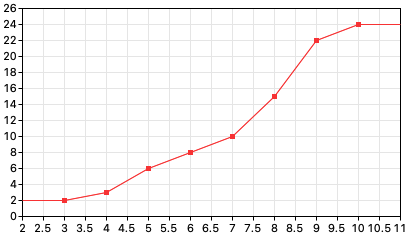
\includegraphics[width=300px ]{Immagini/function.png} 
    \caption{restTime()}
    \label{fig:function}
\end{figure}


Le \textit{resource pool} hanno anch'esse dei valori che possono essere impostati e nel nostro modello ci siamo soffermati in particolare sul numero di elementi che componevano ogni pool che riportiamo:
\begin{itemize}
\item \texttt{Nurses = 10}
\item \texttt{Registrars = 2}
\item \texttt{TriageRooms = 2}: viene impostata in base alle stanze per il triage effettivamente esistenti, nel nostro caso due.
\item \texttt{TicketMachine = 1}
\item \texttt{VisitRooms = 4}: viene impostata in base alle sale visita effettivamente esistenti, nel nostro caso quattro.
\item \texttt{SurgeryRooms = 2}: viene impostata in base alle sale operatorie effettivamente esistenti, nel nostro caso due.
\item \texttt{Beds = 10}
\end{itemize}

\section{Sperimentazioni e Parametri utilizzati} \label{par:esp}

Per poter analizzare propriamente le conseguenze del cambiamento delle variabili sopra descritte, abbiamo definito alcune statistiche che ci permettessero di visualizzare alcune delle metriche più importanti:

\begin{itemize}
    \item \textit{Tempo totale di permanenza, per paziente (minuti)}
    \item \textit{Numero di pazienti presenti nel pronto soccorso, nel tempo}
    \item \textit{Tempo di attesa medio (minuti)}
\end{itemize}

I risultati ottenuti sono stati successivamente confrontati con quelli ottenuti dagli autori dei lavori precedenti (\textit{\cite{espinoza_real-time_2014}}).

Tutte le sperimentazioni sono state eseguite per 500 minuti.

\subsection{Prima sperimentazione} 
I valori dei parametri, per questo primo tentativo, sono stati mantenuti come descritti nei paragrafi precedenti, ovvero arrivano 8 pazienti e 4 ambulanze all'ora. 
Questa sperimentazione sarà utilizzata nel seguito come "caso di default" per i confronti.


Quello che possiamo vedere dall'osservazione di questa iterazione sono i seguenti valori medi riportati in figura \ref{fig:graf1} anche sotto riportati:
\begin{itemize}
    \item \textit{Tempo medio di permanenza:} 163 minuti.
    \item \textit{Numero di pazienti presenti nel pronto soccorso, nel tempo}: 54 pazienti.
    \item \textit{Tempo di attesa medio:} 91 minuti.
\end{itemize}


Possiamo vedere che il numero di pazienti andrebbe ad aumentare così come il tempo medio, e questo potrebbe portare ad una saturazione del pronto soccorso.

\begin{figure}[!h]
    \centering
    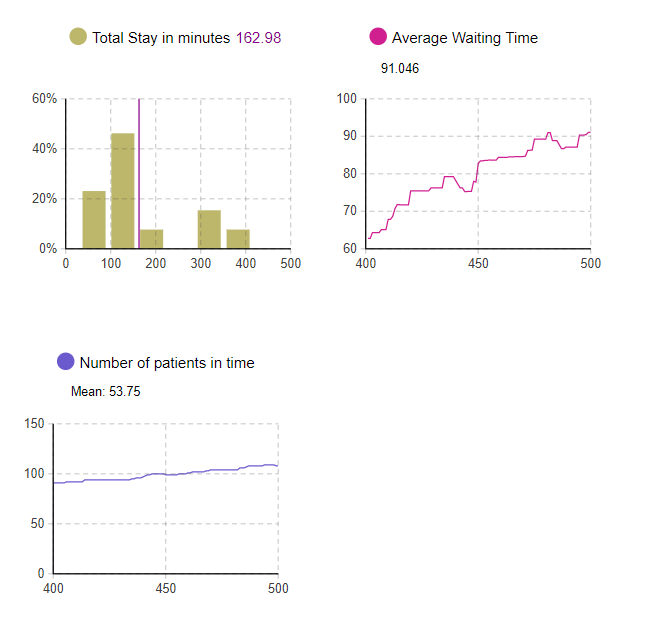
\includegraphics[width=1\textwidth]{Immagini/sper1.png} 
    \caption{Grafici delle metriche della prima sperimentazione}
    \label{fig:graf1}
\end{figure}
\clearpage
\subsection{Seconda Sperimentazione} \label{cahp:seconda}
I valori dei parametri, in questa seconda configurazione, sono stati raddoppiati rispetto alla prima sperimentazione, ovvero arrivano 16 pazienti e 8 ambulanze all'ora. 


Per questa sperimentazione troviamo come valori delle metriche:
\begin{itemize}
    \item \textit{Tempo medio di permanenza:} 221 minuti.
    \item \textit{Numero di pazienti presenti nel pronto soccorso, nel tempo}: 84 pazienti.
    \item \textit{Tempo di attesa medio:} 98 minuti.
\end{itemize}

\subsection{Terza Sperimentazione}
Per eseguire il terzo esperimento abbiamo mantenuto i valori di default per quanto riguarda il tasso di arrivo di ambulanze e pazienti (8 pazienti/ora, 4 ambulanze/ora), modificando però la distribuzione del parametro \textit{sickness} (dei pazienti arrivati a piedi) con una distribuzione uniforme, invece che basarla su percentuali più realistiche come impostato in precedenza. 

Con questa configurazione i risultati ottenuti sono i seguenti: 
\begin{itemize}
    \item \textit{Tempo medio di permanenza:} 143 minuti.
    \item \textit{Numero di pazienti presenti nel pronto soccorso, nel tempo}: 46 pazienti.
    \item \textit{Tempo di attesa medio:} 78 minuti.
\end{itemize}


\subsection{Quarta Sperimentazione}
Per l'esecuzione del quarto esperimento abbiamo scelto di modificare il tempo di attesa nel triage abbassandolo (\texttt{triangular(2, 20, 5)} $\rightarrow$ \texttt{triangular(2, 10, 5)}) e riportare le percentuali di \textit{sickness} su una distribuzione realistica ed abbiamo ottenuto i seguenti risultati.

\begin{itemize}
    \item \textit{Tempo medio di permanenza:} 156 minuti.
    \item \textit{Numero di pazienti presenti nel pronto soccorso, nel tempo}: 53 pazienti.
    \item \textit{Tempo di attesa medio:} 76 minuti.
\end{itemize}

\subsection{Quinta Sperimentazione}
L'ultima sperimentazione effettuata ha previsto l'aumento del numero di infermieri disponibili, da 10 a 20, mantenendo i tassi di arrivo di default. 

I risultati ottenuti sono i seguenti: 
\begin{itemize}
    \item \textit{Tempo medio di permanenza:} 142 minuti.
    \item \textit{Numero di pazienti presenti nel pronto soccorso, nel tempo}: 53 pazienti.
    \item \textit{Tempo di attesa medio:} 89 minuti.
\end{itemize}

\section{Risultati}

In seguito alle sperimentazioni effettuate con i parametri impostati come precedentemente presentato nel paragrafo \ref{par:esp}, abbiamo potuto osservare e trarre le seguenti conclusioni: 

\begin{enumerate}
    \item A parità di tasso di arrivo, una distribuzione uniforme dei codici dei pazienti (per quanto irrealistica) migliora di molto l'efficienza in tutte e tre le metriche analizzate, come prevedibile. Tuttavia non si avrà mai questo caso nella realtà;
    \item La diminuzione del tempo massimo di triage ha un leggero impatto sul tempo di attesa medio, che passa da 91 minuti del caso di default a 76 minuti;
    \item Il raddoppio dei tassi di arrivo adottato nella seconda sperimentazione influisce negativamente in maniera sostanziale sul tempo medio di permanenza, mentre non impatta troppo il tempo di attesa medio;
    \item L'aumento del numero di infermieri disponibili non migliora quasi per nulla l'efficienza rispetto al caso di default. Questo può essere dovuto al fatto che gli infermieri, nel nostro modello, hanno mansioni di solo accompagnamento che difficilmente portano ad una saturazione delle risorse disponibili.  
\end{enumerate}

In conclusione, da quanto osservato, possiamo dire che per aumentare il più possibile l'efficienza del modello e di conseguenza quella di un caso reale, non essendo evidentemente possibile diminuire sempre il tempo massimo di visite e triage o prevedere una distribuzione uniforme della gravità dei pazienti, si potrebbe pensare di aumentare la capacità del pronto soccorso con nuove stanze, permettendo così il trattamento di più pazienti in parallelo. 

È tuttavia da sottolineare che nel presente modello non sono state considerate varie problematiche reali come ad esempio il cambio di turno dello staff o la sua non-disponibilità, che potrebbero peggiorare di molto le metriche prese in considerazione. 

\section{Confronto con lavori precedenti}

I risultati ottenuti nei paper di riferimento per la costruzione del modello non sono perfettamente comparabili con i risultati da noi osservati poiché essi utilizzavano varie distinzioni di scenari maggiormente complessi ed articolati rispetto al nostro lavoro.

Possiamo però sottolineare come in \textit{\cite{espinoza_real-time_2014}} vengano messi in evidenza il numero di accessi al pronto soccorso durante il giorno al variare del giorno della settimana considerato. Valutando una media degli accessi giornalieri possiamo vedere una media che si mantiene tra i 6 e gli 8 pazienti all'ora, con picchi fino a 12 nelle ore più congestionare e 2 nelle ore notturne. Nella nostra simulazione abbiamo provato a simulare un momento di particolare congestione nel paragrafo \ref{cahp:seconda} arrivando a sedici pazienti e quattro ambulanze all'ora. Da notare però che il tempo medio di attesa in tutte queste condizione rimane sostanzialmente inferiore a quello dai noi osservato (dai 10 ai 37 minuti rispetto ai 76-98 del nostro modello).
In merito però a questi risultati possiamo però dire che la simulazione presentata nel paper ha delle differenze sostanziali nella costruzione del pronto soccorso basandosi su una struttura esistente ed i tempi non derivano da una simulazione ma dall'osservazione reale del fenomeno.

Per questo motivo, se pure si è cercato di imitare un contesto realistico e vicino alla realtà, abbiamo comunque scelto di generalizzare piuttosto che andare nello specifico di un singolo pronto soccorso esistente e per questo motivo i dati dei paper non coincidono perfettamente con i nostri.
